\section{SatNOGS-Netzwerk}
\label{sec:sat}
Das SatNOGS-Netzwerk spielt eine zentrale Rolle in unserer Diplomarbeit und bietet hunderten Forschern, Amateurfunkern und Interessierten eine Plattform für verlässliche Kommunikation mit Satelliten.\\
\newline
Das, was SatNOGS zu so einer attraktiven Lösung macht, ist der Fakt dass die Bodenstation um den ganzen Globus verteilt sind. Der große Vorteil davon ist, dass der Empfang von Satellitendaten nun über alle verfügbaren Empfangsstationen laufen kann.\\
\newline
In Abbildung \ref{fig:SatNOGS_Erklärung} wird die Topologie des SatNOGS-Netzwerkes abstrahiert dargestellt.
Alle über das Netzwerk verfügbaren Bodenstationen sind mit SatNOGS-Servern verbunden. Auf diese Server kann über die Website bzw. API zugegriffen werden, welche die empfangenen Satellitendaten für alle Benutzer erreichbar macht.

\begin{figure}[H]
	\centering
	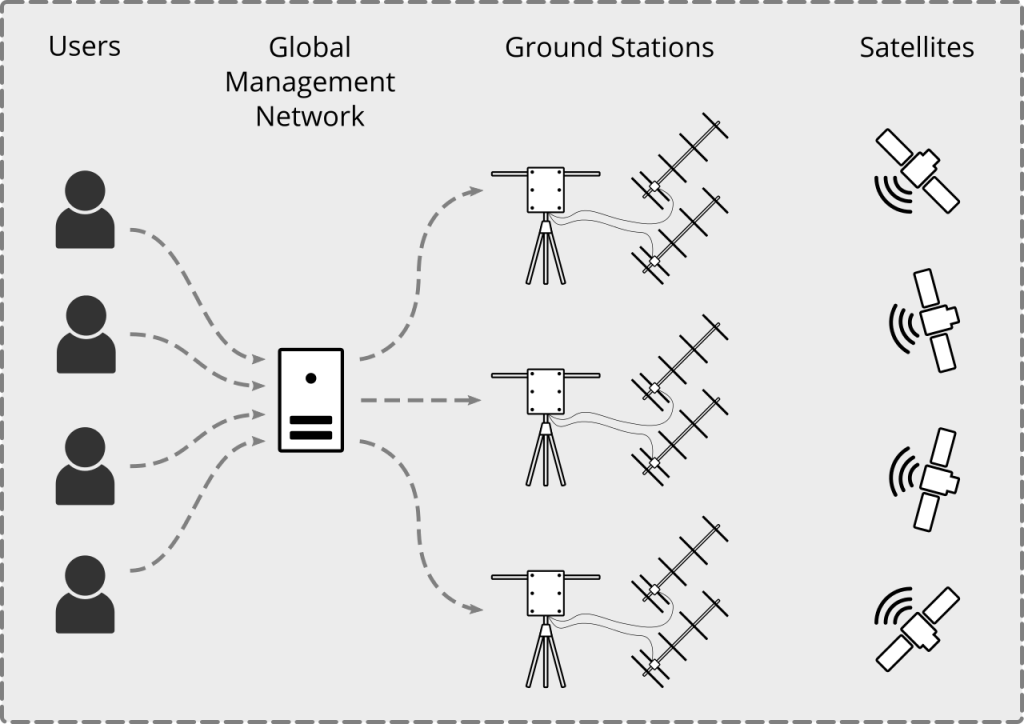
\includegraphics[width=\textwidth]{../ref/SatNOGS_explanation}
	\caption{Erklärung des SatNOGS Netzwerkes}
	\label{fig:SatNOGS_Erklärung}
\end{figure}	

\begin{figure}[H]
	\centering
	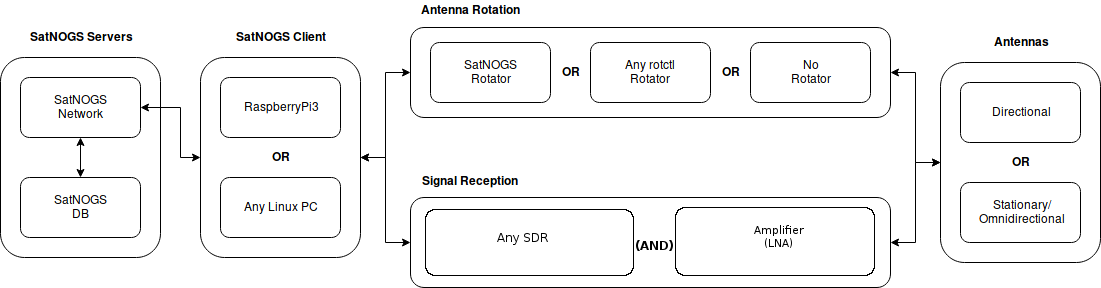
\includegraphics[width=\textwidth]{../ref/SatNOGS_BlockDiagram}
	\caption{SatNOGS-Systemtopologie}
	\label{fig:SatNOGS_Systemtopologie}
\end{figure}

Um näher auf den Ablauf des Datenempfangs und der benötigten Systemblöcke einzugehen wird auf Abbildung \ref{fig:SatNOGS_Systemtopologie} verwiesen.\\
\newline
Zum Empfang von Daten kommen zwei Antennentypen infrage: Direktionale oder omnidirektionale Antennen. Eine direktionale Antenne folgt dem Verlauf des Satelliten. Dies bringt den Vorteil mit sich, dass eine höhere Empfangsleistung erzielt, und somit klarere Daten empfangen werden, jedoch wird für solch ein Modell ein Rotator benötigt. Der Vorteil einer omnidirektionalen Antenne ist, dass kein teurer Rotator notwendig ist, allerdings können damit nur schwer brauchbare Daten empfangen werden.\\
\newline
Für gerichtete Antennen können verschiedene Rotatoren benutzt werden, unter anderem der "SatNOGS-Rotator" sowie diverse Open-Source-Rotatoren und Rotatoren welche zum Verkauf stehen.\\
\newline
Zur Demodulation der Daten sind ein SDR (Software Defined Radio) sowie ein LNA (Low Noise Amplifier) notwendig. Das SDR übernimmt softwaretechnisch Aufgaben welche normalerweise von Hardware übernommen werden (Demodulation, Filter, Mixer, etc...). Der LNA, wie der Name schon andeutet, ist für die Verstärkung kleiner Signale mit besonderer Rauscharmut verantwortlich. \\
\newline
Die Aufgabe des SatNOGS Clients kann in der Regel von jedem Linux-PC oder RaspberryPi übernommen werden. Allerdings wird die Kompatibilität zwar für alle Linux-basierten PCs, jedoch nur für die RaspBerryPis Version 3, 3+ und 4 garantiert.\\
\newline
Der SatNOGS Client ist mit den Servern verbunden, der die Bodentation als solche im Netzwerk repräsentiert. Die Server unterhalten weiters eine Datenbank, welche Daten über Satelliten enthält, die mit den Empfangsstationen erreichbar sind.
\pagebreak